\documentclass[12pt]{Qual}

\usepackage{preamble}

\newtheorem{theorem}{Theorem}
\newtheorem{example}{Example}
\newtheorem{formula}{Formula}
\newtheorem{definition}{Definition}

\name{Kayla Orlinsky}
\course{Complex Analysis Exam}
\term{Complex Analysis}
\hwnum{Cheat Sheet}

\begin{document}
%----------------------%
%----------------------%
\begin{center}
\noindent\textcolor{blue!60!black}{\rule{15cm}{1mm}}
\Huge \faBug\faPuzzlePiece\faCoffee Cauchy Formulas \faCoffee\faPuzzlePiece\faBug
\vspace{-0.5cm}
\noindent\textcolor{blue!60!black}{\rule{15cm}{1mm}}
\end{center}
\vspace{0.5cm}
%----------------------%
%----------------------%
\begin{theorem}{\Large\textit{Cauchy-Riemann Equations}}

\begin{minipage}{0.4\textwidth}
$f(z)=f(x,y)=u(x,y)+iv(x,y)$ is analytic ($C^\infty$) in $\Omega$
\end{minipage}\hspace{1.5cm}\boxed{\iff}\hspace{-1cm}\begin{minipage}{0.4\textwidth}
\hspace{-3.5cm}\vspace{-1cm}
\begin{align*}
    u_x&=v_y\\
    u_y&=-v_x
\end{align*}
\end{minipage}

And $f'(x)=u_x+iv_x$.
\end{theorem}
\vspace{0.5cm}
%----------------------%
%----------------------%
\begin{theorem}{\Large\textit{Cauchy Integral Formula}}

\boxed{\text{\large If:}} $f(z)$ is analytic on open simply connected region $\Omega$ containing $\{|\xi-z|<\rho\}$,

\boxed{\text{\large Then:}} $$f^{(n)}(z)=\frac{n!}{2\pi i}\int_{|\xi-z|<\gamma}\frac{f(\xi)}{(\xi-z)^{n+1}}d\xi$$

\begin{mybox}
***Note that if $f$ is analytic in $\Omega$, then $\displaystyle f(z)=\frac{1}{2\pi i}\int$
\end{mybox}
\end{theorem}
\vspace{0.5cm}
%----------------------%
%----------------------%
\begin{theorem}{\Large\textit{Cauchy Estimate}}

\boxed{\text{\large If:}} $f(z)$ is analytic in $\Omega$ containing $B=\{|\xi-z|<R\}$,

\boxed{\text{\large Then:}} if $\displaystyle M_R=\max_{a\in\partial B}|f(a)|$ then $$|f^{(n)}(z)|\le\frac{n!M_R}{R^n}$$

\end{theorem}
\newpage
%----------------------%
%----------------------%









\begin{center}
\noindent\textcolor{blue!60!black}{\rule{15cm}{1mm}}
\Huge \faBug\faPuzzlePiece\faCoffee Counting Zeros \faCoffee\faPuzzlePiece\faBug
\vspace{-0.5cm}
\noindent\textcolor{blue!60!black}{\rule{15cm}{1mm}}
\end{center}
\vspace{0.5cm}
%----------------------%
%----------------------%
\begin{theorem}{\Large\textit{Rouche's}}

\boxed{\text{\large If:}}
\vspace{-0.25cm}
\begin{itemize}[leftmargin=2.5cm]
\setlength\itemsep{-0.1em}
\renewcommand\labelitemi{\faPuzzlePiece}
    \item $f$ and $g$ are analytic in $\Omega$ containing a closed curve $\Gamma$
    \item $|f(z)-g(z)|<|f(z)|$ or $|f(z)-g(z)|<|g(z)|$ for all $z\in\Gamma$,
\end{itemize}

\boxed{\text{\large Then:}} $f$ and $g$ have the same number of zeros inside $\Gamma$.

\begin{mybox}
***Alternatively, if $|g(z)|<|f(z)|$ on $\Gamma$, then $f$ and $f+g$ have the same number of zeros inside $\Gamma.$
\end{mybox}
\end{theorem}
\vspace{-0.5cm}
%----------------------%
%----------------------%
\begin{theorem}{\Large\textit{Argument Principle}}

\boxed{\text{\large If:}} \begin{minipage}{0.85\textwidth}
\vspace{0.45cm}
$f$ is meromorphic in $\Omega$ and $\Gamma\subset\Omega$ has winding number $1$ and avoids zeros and poles of $f$,
\end{minipage}

\boxed{\text{\large Then:}}
then $$\frac{1}{2\pi i}\int_\Gamma\frac{f'(z)}{f(z)}dz=\#\text{zeros}-\#\text{poles}\qquad\text{enclosed by }\Gamma.$$

\end{theorem}
%----------------------%
%----------------------%
\begin{example}
$\,$
\begin{framed}
Find the number of solutions of the equation $z-2-e^{-z}=0$ in $H=\{z\in\mathbb{C}:\re(z)>0\}.$
\end{framed}
Let $f(z)=z-2-e^{-z}$. Then $f(iy)=iy-2-e^{-iy}=-2-\cos(y)+i(y-\sin(y)).$
Thus, $\re(f(iy))<0$ for all $y\in\mathbb{R}$ and $f$ sends the imaginary axis to the left-half plane, away from the origin.

On a large half-circle in the right-half plane, $z=Re^{i\theta}$ for $\theta\in(-\pi/2,\pi/2)$ and $$\frac{1}{R}f(Re^{i\theta})=e^{i\theta}-\frac{2}{R}-\frac{e^{-Re^{i\theta}}}{R}\to e^{i\theta}\qquad R\to\infty.$$ Therefore, $f$ has a total change in argument of $\pi$ so $f$ can have at most one zero in the right half plane.

Since $f(0)<0$ and $f(10)=8-\frac{1}{e^{10}}>7>0$ by the intermediate value theorem, $f$ has a zero on the positive real axis so $f$ has exactly one zero in the right-half plane.
\end{example}

%----------------------%
%----------------------%
\newpage







\begin{center}
\noindent\textcolor{blue!60!black}{\rule{15cm}{1mm}}
\Huge \faBug\faPuzzlePiece\faCoffee Bounded Functions \faCoffee\faPuzzlePiece\faBug
\vspace{-0.5cm}
\noindent\textcolor{blue!60!black}{\rule{15cm}{1mm}}
\end{center}
\vspace{0.25cm}
%----------------------%
%----------------------%
\begin{theorem}{\Large\textit{Louiville}}

\boxed{\text{\large If:}} $f(z)$ is entire and bounded

\boxed{\text{\large Then:}} $f(z)$ is constant

\end{theorem}
\vspace{0.25cm}
%----------------------%
%----------------------%
\begin{theorem}{\Large\textit{Schwarz'}}

\boxed{\text{\large If:}} $f:\mathbb{D}\to\mathbb{D}$ ($\mathbb{D}=\{|z|<1\}$)
\vspace{-0.25cm}
\begin{itemize}[leftmargin=2.5cm]
\setlength\itemsep{-0.1em}
\renewcommand\labelitemi{\faPuzzlePiece}
    \item analytic
    \item $f(0)=0$
\end{itemize}

\boxed{\text{\large Then:}} $|f(z)|\le|z|$ on $\mathbb{D}$ and $|f'(0)|\le 1$.

\begin{mybox}
***If, additionally $|f(z)|=|z|$ for some $z\not=0$ \textit{or} if $|f'(0)|=1$, then $f(z)=az$ for some $|a|=1$.
\end{mybox}

\end{theorem}
\vspace{0.25cm}
%----------------------%
%----------------------%
\begin{theorem}{\Large\textit{Maximum Modulus Principle}}

\boxed{\text{\large If:}} \begin{minipage}{0.85\textwidth}
\vspace{0.45cm}
If $f$ is analytic in an open simply connected set $\Omega$, and $f$ has a maximum value inside $\Omega$
\end{minipage}

\boxed{\text{\large Then:}} $f$ is constant.

***Namely, analytic function must attain their maximum on the boundary of any simply connected set.

\end{theorem}
\vspace{0.25cm}
%----------------------%
%----------------------%
\begin{theorem}{\Large\textit{Schwarz Reflection Principle}}

\boxed{\text{\large If:}}
\vspace{-0.25cm}
\begin{itemize}[leftmargin=2.5cm]
\setlength\itemsep{-0.1em}
\renewcommand\labelitemi{\faPuzzlePiece}
    \item $f$ is analytic in the upper half plane,
    \item $f$ is continuous on the real line and $f(x)\in\mathbb{R}$ for all $x\in\mathbb{R}$ ($f$ is real on the real line)
\end{itemize}

\boxed{\text{\large Then:}} \begin{minipage}{0.85\textwidth}
\vspace{0.45cm}
$f$ can be extended to an analytic function on the negative half plane by the formula $f(\overline{z})=\overline{f(z)}.$
\end{minipage}



\end{theorem}
%----------------------%
%----------------------%
\newpage



















\begin{center}
\noindent\textcolor{blue!60!black}{\rule{15cm}{1mm}}
\Huge \faBug\faPuzzlePiece\faCoffee Residues \faCoffee\faPuzzlePiece\faBug
\vspace{-0.5cm}
\noindent\textcolor{blue!60!black}{\rule{15cm}{1mm}}
\end{center}
\vspace{0.5cm}
%----------------------%
%----------------------%
\begin{theorem}{\Large\textit{Residue Theorem}}

\boxed{\text{\large If:}}
\vspace{-0.25cm}
\begin{itemize}[leftmargin=2.5cm]
\setlength\itemsep{-0.1em}
\renewcommand\labelitemi{\faPuzzlePiece}
    \item $\Gamma\subset\Omega$ closed curve
    \item $\Omega$ open and simply connected,
    \item $f(z)$ is a meremorphic function in $\Omega$
    \item $\Gamma$ intersects no poles of $f$
\end{itemize}

\boxed{\text{\large Then:}} if $\Gamma$ encloses $\{a_1,...,a_n\}$ poles of $f,$ $$\int_\Gamma f(z)dz=2\pi i\sum_{j=1}^n\res_{z=a_j}f(z)$$

\end{theorem}
\vspace{0.5cm}
%----------------------%
%----------------------%
\begin{formula}{\Large\textit{Residue Formula}}
If $a$ is a pole of order $n$ of $f(z)$, then
$$\res_{z=a}f(z)=\lim_{z\to a}\frac{1}{(n-1)!}\frac{d^{n-1}}{dz^{n-1}}((z-a)^nf(z)).$$

***The residue of $f(z)$ at $a$ is exactly the coefficient of the $\frac{1}{z}$ term in the Laurent expansion of $f(z)$ at $a.$
\end{formula}
\vspace{0.5cm}
%----------------------%
%----------------------%
\begin{example}
$\,$
\begin{framed}
Evaluate $$\int_0^{2\pi}\frac{d\theta}{3+\cos\theta+2\sin\theta}.$$
\end{framed}
\begin{align*}
    \int_0^{2\pi}\frac{d\theta}{3+\cos\theta+2\sin\theta}&=\int_0^{2\pi}\frac{d\theta}{3+\frac{e^{i\theta}+e^{-i\theta}}{2}+\frac{e^{i\theta}-e^{-i\theta}}{i}}\\
    &=\int_0^{2\pi}\frac{2ie^{i\theta}d\theta}{6ie^{i\theta}+ie^{2i\theta}+i+2e^{2i\theta}-2}\\
    &=\int_{|z|=1}\frac{2dz}{6iz+iz^2+i+2z^2-2}\qquad z=e^{i\theta}\\
    &=\int_{|z|=1}\frac{2dz}{(i+2)z^2+6iz+i-2}\\
    &=\int_{|z|=1}\frac{2dz}{(i+2)\left(z+\frac{1}{5}(1+2i)\right)(z+1+2i)}\tag{1}\\
    &=\left(2\pi i\res_{z=-\frac{1}{5}(1+2i)}\frac{2}{(i+2)\left(z+\frac{1}{5}(1+2i)\right)(z+1+2i)}\right)\tag{2}\\
    &=2\pi i \frac{2}{(i+2)\left(-\frac{1}{5}(1+2i)+1+2i\right)}\\
    &=4\pi i\frac{1}{(i+2)\frac{4}{5}(1+2i)}\\
    &=5\pi i\frac{1}{(1+2i)(i+2)}\\
    &=5\pi i\frac{1}{i+2-2+4i}\\
    &=5\pi i\frac{1}{5i}\\
    &=\pi
\end{align*}

Where (1) comes from the quadratic formula, and (2) because only one pole is contained in the unit disk.
\end{example}
\vspace{0.5cm}
%----------------------%
%----------------------%
\begin{example}
$\,$
\begin{framed}
Evaluate the integral $$\int_0^\infty\frac{dx}{1+x^n},\qquad n\ge2.$$
\end{framed}

Then we get that there is a pole at $e^{i\frac{\pi}{n}}$ which can be isolated in a pizza slice of angle $\frac{2\pi}{n}$.

Thus, we integrate around the following contour:
\begin{center}
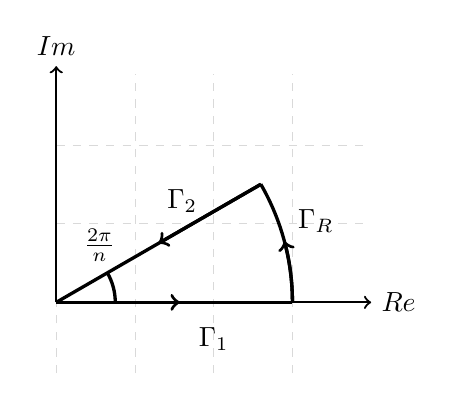
\begin{tikzpicture}
\draw[help lines, color=gray!30, dashed] (0,-0.9) grid (3.9,2.9);
\draw[->,very thick] (3,0) arc (0:15:3cm);
\draw[very thick] (3,0) arc (0:30:3cm) node[above,yshift=-0.75cm,xshift=0.7cm]{$\Gamma_R$};
\draw[->,very thick] (0,0) -- (1.57,0);
\draw[very thick] (0.75,0) -- (3,0) node[above,yshift=-0.75cm,xshift=-1cm]{$\Gamma_1$};
\draw[->,very thick] (2.6,1.5) -- (1.3,0.75);
\draw[very thick] (0,0) -- (2.6,1.5) node[above,yshift=-0.5cm,xshift=-1cm]{$\Gamma_2$};
\draw[very thick] (0.75,0) arc (0:30:0.75cm) node[above,yshift=0cm,xshift=-0.1cm]{$\frac{2\pi}{n}$};
\draw[->, thick] (0,0)--(4,0) node[right]{$Re$};
\draw[->, thick] (0,0)--(0,3) node[above]{$Im$};
\end{tikzpicture}
\end{center}

Immeidately, we get that $$|I_R|=\left|\int_{\Gamma_R}\frac{dz}{1+z^n}\right|\le\int_0^{\frac{2\pi}{n}}\frac{R}{R^n-1}d\theta=\frac{2\pi R}{n(R^n-1)}\to0\qquad R\to\infty.$$

Since $$I_2=\int_{\Gamma_2}\frac{dz}{1+z^n}=\int_R^0\frac{e^{i\frac{2\pi}{n}}dr}{1+r^ne^{2\pi i}}=-e^{i\frac{2\pi}{n}}\int_0^R\frac{dr}{1+r^n}=-e^{i\frac{2\pi}{n}}I_1.$$

Thus, using the residue theorem, we get that $$\res_{z=e^{i\frac{\pi}{n}}}\frac{1}{1+x^n}=\lim_{z\to e^{i\frac{\pi}{n}}}\frac{x-e^{i\frac{\pi}{n}}}{x^n+1}=\lim_{z\to e^{i\frac{\pi}{n}}}\frac{1}{nx^{n-1}}=\frac{1}{n}e^{-(n-1)i\frac{\pi}{n}}$$ and that $$2\pi i\frac{1}{n}e^{-(n-1)i\frac{\pi}{n}}=\lim_{R\to\infty}(I_1+I_2+I_R)=(1-e^{i\frac{2\pi}{n}})I_1$$ and so $$\int_0^\infty\frac{dx}{1+x^n}= \frac{\pi}{n}e^{-(n-1)i\frac{\pi}{n}}\frac{2i}{1-e^{i\frac{2\pi}{n}}}=\frac{\pi}{n}\frac{-2i}{e^{-i\frac{\pi}{n}}-e^{i\frac{\pi}{n}}}=\frac{\pi/n}{\sin(\pi/n)}$$
\end{example}
\newpage






\begin{center}
\noindent\textcolor{blue!60!black}{\rule{15cm}{1mm}}
\Huge \faBug\faPuzzlePiece\faCoffee Harmonic and Subharmonic \faCoffee\faPuzzlePiece\faBug
\vspace{-0.5cm}
\noindent\textcolor{blue!60!black}{\rule{15cm}{1mm}}
\end{center}
\vspace{0.5cm}
%----------------------%
%----------------------%
\begin{definition}{\Large\textit{Harmonic Function}}

$u:\Omega\to\mathbb{R}$ where $\Omega$ is open and could be real or complex is harmonic if its Laplacian is zero: $$u_{xx}+u_{yy}=0.$$

\end{definition}
\vspace{0.5cm}
%----------------------%
%----------------------%
\begin{theorem}{\Large\textit{Maximum and Minimum Principle}}

\boxed{\text{\large If:}}\begin{minipage}{0.85\textwidth}
\vspace{0.45cm}
$u$ is harmonic on an open simply connected set $\Omega$ and $u$ attains a maximum \textit{or} minimum value inside $\Omega$
\end{minipage}


\boxed{\text{\large Then:}} $u$ is constant

***harmonic functions attain their maximum \textit{and} minimum values on the boundary of open sets.
\end{theorem}
\vspace{0.5cm}
%----------------------%
%----------------------%
\begin{theorem}{\Large\textit{Mean Value Property}}

\boxed{\text{\large If:}} $u$ is harmonic on an open set $\Omega$,

\boxed{\text{\large Then:}} for each $z_0\in\Omega$ and $r>0$ such that $\overline{B_r(z_0)}=\{|z-z_0|\le r\}\subset\Omega$, $$u(z_0)=\frac{1}{2\pi}\int_0^{2\pi}u(z_0+re^{i\theta})d\theta.$$

\end{theorem}
\vspace{0.5cm}
%----------------------%
%----------------------%
\begin{theorem}{\Large\textit{Poisson Formula}}

\boxed{\text{\large If:}} $u$ is harmonic on an open set $\Omega$ and $\overline{\mathbb{D}}=\{|z|\le1\}\subset\Omega$,

\boxed{\text{\large Then:}} for all $|z|<1$, $$u(z)=\frac{1}{2\pi}\int_0^{2\pi}\frac{1-|z|^2}{|e^{i\theta}-z|^2}u(e^{i\theta})d\theta.$$

***The Poisson Kernel is $\displaystyle\frac{|\xi|^2-|z|^2}{|\xi-z|^2}$.

\end{theorem}
\vspace{0.5cm}
%----------------------%
%----------------------%
\begin{theorem}{\Large\textit{Harnack's Inequality}}

\boxed{\text{\large If:}} $u$ is a \textit{non-negative} analytic inside $B_R(z_0)$ and continuous on the boundary,

\boxed{\text{\large Then:}} for all $r<R$, $$\frac{R-r}{R+r}u(z_0)\le u(z)\le\frac{R+r}{R-r}u(z_0).$$

\end{theorem}
\vspace{0.5cm}
%----------------------%
%----------------------%
\begin{definition}{\Large\textit{Subharmonic Function}}

$v:\Omega\to\mathbb{R}$ where $\Omega$ is open and could be real or complex is subharmonic if its Laplacian is non-negative: $$u_{xx}+u_{yy}\ge0.$$

\end{definition}
\vspace{0.5cm}
%----------------------%
%----------------------%
\begin{theorem}{\Large\textit{Maximum Principle for Subharmonic Functions}}

\boxed{\text{\large If:}}
$v$ is subharmonic in $\Omega$, and $u$ is any harmonic function in $\Omega$

\boxed{\text{\large Then:}} \begin{minipage}{0.85\textwidth}
\vspace{0.45cm}
$u-v$ has the maximum principle (but not necessarily the minimum principle).
\end{minipage}

\end{theorem}
\vspace{0.5cm}
%----------------------%
%----------------------%
\begin{theorem}{\Large\textit{MVP for Subharmonic Functions}}

\boxed{\text{\large If:}}
$v$ is subharmonic on $\Omega$

\boxed{\text{\large Then:}} for each $z_0\in\Omega$ and $r>0$ such that $\overline{B_r(z_0)}=\{|z-z_0|\le r\}\subset\Omega$, $$v(z_0)\le \frac{1}{2\pi}\int_0^{2\pi}u(z_0+re^{i\theta})d\theta.$$

\end{theorem}
\vspace{0.5cm}
%----------------------%
%----------------------%
\newpage







\begin{center}
\noindent\textcolor{blue!60!black}{\rule{15cm}{1mm}}
\Huge \faBug\faPuzzlePiece\faCoffee Infinite Series and Products \faCoffee\faPuzzlePiece\faBug
\vspace{-0.5cm}
\noindent\textcolor{blue!60!black}{\rule{15cm}{1mm}}
\end{center}
\vspace{0.5cm}
%----------------------%
%----------------------%
\begin{theorem}{\Large\textit{Taylor's}}

\begin{minipage}{0.4\textwidth}
$f(z)$ is analytic at a point $z_0$
\end{minipage}\boxed{\iff}\hspace{0.5cm}\begin{minipage}{0.4\textwidth}
There exists a neighborhood $U$ of $z_0$ such that $f$ has a convergent Taylor Series at $z_0$ in $U.$
\end{minipage}
\vspace{0.5cm}

The Taylor Series is unique and converges uniformly on compact subsets.
\end{theorem}
\vspace{0.25cm}
%----------------------%
%----------------------%
\begin{theorem}{\Large\textit{Laurent}}

\begin{minipage}{0.4\textwidth}
$f(z)$ has an isolated singularity at $z_0$
\end{minipage}\hspace{0.5cm}\boxed{\iff}\hspace{0.5cm}\begin{minipage}{0.4\textwidth}
There exists Laurent series at $z_0$ which converges in some annulus avoiding $z_0$.
\end{minipage}
\vspace{0.5cm}

The Laurent Series is unique and converges uniformly on compact subsets.
\end{theorem}
\vspace{0.25cm}
%----------------------%
%----------------------%
\begin{theorem}{\Large\textit{Convergence Criterion for Infinite product}}

\begin{minipage}{0.4\textwidth}
$\displaystyle \prod_{n=1}^\infty a_n$ converges
\end{minipage}\boxed{\iff}\hspace{0.5cm}\begin{minipage}{0.4\textwidth}
$\displaystyle\sum_{n=1}^\infty\log(a_n)$ converges for some branch cut of $\log.$
\end{minipage}
\vspace{0.5cm}

\begin{minipage}{0.4\textwidth}
$\displaystyle \prod_{n=1}^\infty(1+a_n)$ converges absolutely
\end{minipage}\boxed{\iff}\hspace{0.5cm}\begin{minipage}{0.4\textwidth}
$\displaystyle\sum_{n=1}^\infty|a_n|$ converges
\end{minipage}
\vspace{0.5cm}

\end{theorem}
\vspace{0.25cm}
%----------------------%
%----------------------%
\begin{theorem}{\Large\textit{Analyticitiy of an Infinite product}}

\begin{minipage}{0.4\textwidth}
$\displaystyle \prod_{n=1}^\infty f_n(z)$ represents an analytic function
\end{minipage}\hspace{0.5cm}\boxed{\iff}\hspace{0.5cm}\begin{minipage}{0.4\textwidth}
$\displaystyle \prod_{n=1}^\infty f_n(z)$ converges uniformly on compact subsets.
\end{minipage}
\vspace{0.5cm}

\begin{minipage}{0.4\textwidth}
$\displaystyle \prod_{n=1}^\infty f_n(z)$ converges uniformly on compact subsets
\end{minipage}\hspace{0.5cm}\boxed{\iff}\hspace{0.5cm}\begin{minipage}{0.4\textwidth}
$\displaystyle\sum_{n=1}^\infty|f_n(z)-1|$ converges uniformly on compact subsets
\end{minipage}

\end{theorem}
\vspace{0.5cm}
%----------------------%
%----------------------%
\begin{theorem}{\Large\textit{Weierstrauss $M$-test}}

\boxed{\text{\large If:}}\hspace{0.1cm}\begin{minipage}{0.85\textwidth}
\vspace{0.45cm}
there exists a sequence $\{M_n\}_{n=1}^\infty\subset\mathbb{R}^+$ ($M_n\ge0$ for all $n$) such that $|f_n(z)|\le M_n$ for all $n$
\end{minipage}

\boxed{\text{\large Then:}} $\displaystyle\sum_{n=1}^\infty f_n(z)$ converges absolutely and uniformly on compact subsets.

\end{theorem}
\vspace{0.5cm}
%----------------------%
%----------------------%
\begin{definition}{\Large\textit{Radius of Convergence}}

The radius of convergence $R$ of a series (Taylor or otherwise) $\displaystyle\sum_{n=1}^\infty a_n(z-z_0)^n$ is given by the formula $\displaystyle\frac{1}{R}=\limsup_{n\to\infty}|a_n|^{1/n}$

\end{definition}
\vspace{0.5cm}
%----------------------%
%----------------------%
\begin{formula}{\Large\textit{Taylor Series}}
\vspace{-0.5cm}
\begin{center}
    $$\begin{matrix}
    \text{\faBug} & \displaystyle\frac{1}{1-z} &=\displaystyle\sum_{n=0}^\infty z^n &\qquad |z|<1\\[0.5cm]
   \text{\faBug} & \displaystyle e^z & =\displaystyle\sum_{n=0}^\infty\frac{z^n}{n!} &\\[0.5cm]
    \text{\faBug} & \displaystyle \log(1-z) & =\displaystyle\sum_{n=1}^\infty\frac{z^n}{n} &\qquad |z|<1\\[0.5cm]
   \text{\faBug} & \displaystyle \sin(z) & \qquad=\displaystyle\sum_{n=0}^\infty\frac{z^{2n+1}}{(2n+1)!} &\\[0.5cm]
     \text{\faBug} & \displaystyle \cos(z) & =\displaystyle\sum_{n=0}^\infty\frac{z^{2n}}{(2n)!} &\\[0.5cm]
    \end{matrix}$$
\end{center}

\end{formula}
\vspace{0.5cm}
%----------------------%
%----------------------%
\begin{example}
$\,$
\begin{framed}
Write an entire function which has the simple zeros $1,4,9,16,25,...$ and has no other zeros.
\end{framed}
The zeros are $1^2,2^2,3^2,4^2,5^2,...$. Then let $$f(z)=\prod_{n=1}^\infty\frac{(z-n^2)}{n^2}=\prod_{n=1}^\infty\left(\frac{z}{n^2}-1\right)=-\prod_{n=1}^\infty\left(1-\frac{z}{n^2}\right)$$ Since for all $z$, there exists $M$ so $|z|<M$, we have that $\frac{|z|}{n^2}<\frac{M}{n^2}$ and so $$\sum_{n=1}^\infty\frac{|z|}{n^2}$$ converges uniformly on compact subsets. Therefore, $f$ is entire.
\end{example}
\vspace{0.5cm}
%----------------------%
%----------------------%
\begin{example}
Let $$f(z)=\frac{1}{z(z+1)}.$$ Then $f$ has singularities at $-1$ and $0$. Namely, $f(z)$ will have a Laurent series expansion for $0<|z|<1$ and for $|z|>1$.
\begin{center}
\begin{minipage}{0.4\textwidth}
\vspace{-1.75cm}
On $0<|z|<1$, \begin{align*}
    f(z)&=\frac{1}{z(z+1)}\\
    &=\frac{1}{z}-\frac{1}{z+1}\\
    &=\frac{1}{z}-\frac{1}{1-(-z)}\\
    &=\frac{1}{z}-\sum_{n=0}^\infty(-z)^n\\
    &=\sum_{n=-1}^\infty(-1)^{n+1}\frac{1}{z^n}
\end{align*}
\end{minipage}\begin{minipage}{0.4\textwidth}
\vspace{0.25cm}
On $|z|>1$, $\frac{1}{|z|}<1$, so \begin{align*}
    f(z)&=\frac{1}{z(z+1)}\\
    &=\frac{1}{z}-\frac{1}{z+1}\\
    &=\frac{1}{z}-\frac{1}{z(1+\frac{1}{z})}\\
    &=\frac{1}{z}-\frac{1}{z}\frac{1}{1-\left(-\frac{1}{z}\right)}\\
    &=\frac{1}{z}-\frac{1}{z}\sum_{n=0}^\infty(-1)^n\frac{1}{z^n}\\
    &=\frac{1}{z}+\sum_{n=0}^\infty(-1)^{n+1}\frac{1}{z^{n+1}}\\
    &=\sum_{n=2}^\infty(-1)^n\frac{1}{z^n}
\end{align*}
\end{minipage}
\end{center}

Now, if we were being asked to find the Laurent Expansion on $\{1<|z-1|<2\}$, then we would be being asked to find the expansion at $a=1.$ Since on $\{1<|z-1|<2\}$ we have that $1>\frac{1}{|z-1|}>\frac{1}{2}$ and $\frac{|z-1|}{2}<1$ so \begin{align*}
    \frac{1}{z(z+1)}&=\frac{1}{z}-\frac{1}{z+1}\\
    &=\frac{1}{(z-1)+1}-\frac{1}{(z-1)+2}\\
    &=\frac{\frac{1}{z-1}}{1+\frac{1}{z-1}}-\frac{\frac{1}{2}}{1+\frac{z-1}{2}}\\
    &=\frac{1}{z-1}\frac{1}{1-\frac{1}{1-z}}-\frac{1}{2}\frac{1}{1-\frac{1-z}{2}}\\
    &=\frac{1}{z-1}\sum_{l=0}^\infty\left(\frac{1}{1-z}\right)^l-\frac{1}{2}\sum_{k=0}^\infty\left(\frac{1-z}{2}\right)^k\\
    &=\sum_{l=0}^\infty\frac{1}{(1-z)^{l+1}}-\sum_{k=0}^\infty\frac{(1-z)^k}{2^{k+1}}
\end{align*}
\end{example}

\newpage
%----------------------%
%----------------------%








\begin{center}
\noindent\textcolor{blue!60!black}{\rule{15cm}{1mm}}
\Huge \faBug\faPuzzlePiece\faCoffee Singularities \faCoffee\faPuzzlePiece\faBug
\vspace{-0.5cm}
\noindent\textcolor{blue!60!black}{\rule{15cm}{1mm}}
\end{center}
\vspace{0.5cm}
\begin{definition}{\Large\textit{Singularities}}
\begin{itemize}
\renewcommand\labelitemi{\faCoffee}
    \item \textbf{Exceptional Point:} $\displaystyle\lim_{z\to a}(z-a)f(z)=0$.
    \item \textbf{Zeros:} $f(a)=0$, there exists $k$ and $g$ analytic (and nonzero at $a$) such that $f(z)=(z-a)^kg(z)$.
    \item \textbf{Poles:} $|f(a)|=\infty$, there exists a $k$ and $g$ analytic such that $\displaystyle f(z)=\frac{g(z)}{(z-a)^k}$.
    \item \textbf{Essential Singularity:} Any isolated singularity that is not a pole and is not removable.
\end{itemize}


***Exceptional points are exactly removable singularities. Namely, if $f(z)$ has an exceptional point, it can be extended to an analytic function at that point.

***If $f(z)$ has any type of removable singularity at $\infty$, then $f(1/z)$ has a singularity of the \textit{same type} at $0.$


\end{definition}
\vspace{0.5cm}
%----------------------%
%----------------------%
\begin{theorem}{\Large\textit{Picard's Little Theorem}}

\boxed{\text{\large If:}} $f(z)$ is entire and non-constant

\boxed{\text{\large Then:}} $f$ assumes all but at most $1$ point in $\mathbb{C}$.

\end{theorem}
\vspace{0.5cm}
%----------------------%
%----------------------%
\begin{theorem}{\Large\textit{Picard's Great Theorem}}

\boxed{\text{\large If:}} $f(z)$ has an essential singularity $z_0$,

\boxed{\text{\large Then:}} for every punctured neighborhood $U$ of $z_0$, $f(z)$ for $z\in U$ assumes all but at most $2$ points in $\mathbb{C}\cup\{\infty\}$ infinitely often.

\end{theorem}
\vspace{0.5cm}
%----------------------%
%----------------------%

\newpage










\begin{center}
\noindent\textcolor{blue!60!black}{\rule{15cm}{1mm}}
\Huge \faBug\faPuzzlePiece\faCoffee Normal Families \faCoffee\faPuzzlePiece\faBug
\vspace{-0.5cm}
\noindent\textcolor{blue!60!black}{\rule{15cm}{1mm}}
\end{center}
\vspace{0.5cm}
\begin{definition}{\Large\textit{Singularities}}

If $\mathscr{F}$ is a family (set) of holomorphic functions $f:\Omega\to\mathbb{C}$ is called \textit{normal} if for every sequence $\{f_n\}_{n=1}^\infty\subset\mathscr{F}$ there exists a subsequence $\{f_{n_k}\}_{k=1}^\infty$ which converges uniformly on compact subsets of $\Omega$.

\vspace{0.5cm}

***Note that any sequence of holomorphic functions converging uniformly must converge to a holomorphic function.

\end{definition}
\vspace{0.5cm}
%----------------------%
%----------------------%
\begin{theorem}{\Large\textit{Montel's}}

If $\mathscr{F}$ is a family of holomorphic functions on an open set $\Omega$, then
\vspace{0.25cm}

\begin{minipage}{0.2\textwidth}
$\mathscr{F}$ is normal
\end{minipage}\hspace{-0.25cm}\boxed{\iff}\hspace{0.5cm}\begin{minipage}{0.6\textwidth}
$\mathscr{F}$ is locally uniformly bounded

(for each compact subset $K$ of $\Omega$, there exists $M$ so $|f(z)|\le M$ for all $z\in K$ and for all $f\in\mathscr{F}$)
\end{minipage}

\end{theorem}
\vspace{0.5cm}
%----------------------%
%----------------------%

\newpage








\begin{center}
\noindent\textcolor{blue!60!black}{\rule{15cm}{1mm}}
\Huge \faBug\faPuzzlePiece\faCoffee Conformal Mapping \faCoffee\faPuzzlePiece\faBug
\vspace{-0.5cm}
\noindent\textcolor{blue!60!black}{\rule{15cm}{1mm}}
\end{center}
\vspace{0.25cm}
%----------------------%
%----------------------%
\begin{definition}{\Large\textit{Conformal Map}}

A map $f$ on an open region $\Omega$ is conformal if
\begin{itemize}
\renewcommand\labelitemi{\faCoffee}
    \item $f$ is analytic on $\Omega$
    \item $f'(z)\not=0$ for all $z\in\Omega$
\end{itemize}

***Conformal maps are angle preserving.
\end{definition}
%----------------------%
%----------------------%
\begin{theorem}{\Large\textit{Identity Theorem}}

\boxed{\text{\large If:}} \begin{minipage}{0.85\textwidth}
\vspace{0.45cm}
 $f,g:\Omega\to\mathbb{C}$ where $\Omega$ is open and simply connected and $f=g$ on some subset $S\subset\Omega$ having an accumulation point in $\Omega$
\end{minipage}


\boxed{\text{\large Then:}} $f=g$ on all of $\Omega.$

\end{theorem}
\vspace{0.25cm}
%----------------------%
%----------------------%
\begin{theorem}{\Large\textit{Open Mapping Theorem}}

\boxed{\text{\large If:}} $f$ is analytic

\boxed{\text{\large Then:}}\begin{minipage}{0.85\textwidth}
\vspace{0.45cm}
the image of any open set under $f$ is also open ($f$ sends open sets to open sets).
\end{minipage}



\end{theorem}
\vspace{0.25cm}
%----------------------%
%----------------------%
\begin{theorem}{\Large\textit{Riemann Mapping Theorem}}

\boxed{\text{\large If:}} $\Omega\subset\mathbb{C}$ is
\vspace{-0.25cm}
\begin{itemize}[leftmargin=2.5cm]
\setlength\itemsep{-0.1em}
\renewcommand\labelitemi{\faPuzzlePiece}
    \item open,
    \item simply connected,
    \item and not all of $\mathbb{C}$ ($\Omega$ lacks at least one point of $\mathbb{C}$ or lacks at least two points of $\overline{\mathbb{C}}$)
\end{itemize}
\vspace{-1cm}

\boxed{\text{\large Then:}} \begin{minipage}{0.85\textwidth}
\vspace{1.4cm}
For each $\alpha\in\Omega$ there exists a unique conformal biholomorphic (bijective, analytic, with analytic inverse) function $$g:\Omega\to\mathbb{D}=\{|z|<1\}\qquad g(\alpha)=0$$
\end{minipage}



\end{theorem}
\vspace{0.25cm}
%----------------------%
%----------------------%
\begin{definition}{\Large\textit{Cross Ratio}}

The cross ratio
$$(z,w_2,w_3,w_4)=\frac{z-w_3}{z-w_4}:\frac{w_2-w_3}{w_2-w_4}.$$

And
$$T(z)=\frac{z-w_3}{z-w_4}:\frac{w_2-w_3}{w_2-w_4}$$ is the unique transformation sending $w_2\mapsto 1$, $w_3\mapsto 0$, $w_4\mapsto\infty$.

\end{definition}
%----------------------%
%----------------------%
\begin{formula}{\Large\textit{Conformal Maps}}

\begin{center}
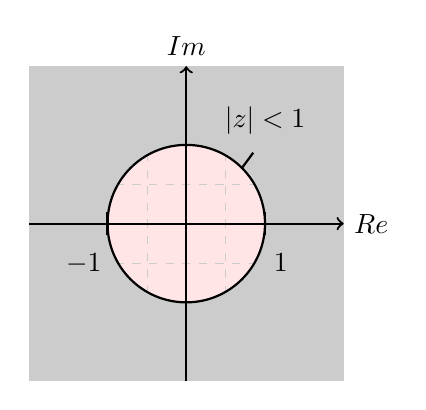
\begin{tikzpicture}[thick,scale=0.5]
\fill[gray!40,even odd rule] (-4,-4) rectangle (4,4);
\fill[red!10,even odd rule] (0,0) circle (2cm);
\draw[help lines, color=gray!40, dashed] (-3.9,-3.9) grid (3.9,3.9);
\draw[thick] (0, 0) circle (2cm) node[above,xshift=1cm,yshift=1cm]{$|z|<1$};
\draw (1.42,1.42) -- (1.7,1.8);
\draw[thick] (2,-0.3) -- (2,0.3) node[below,xshift=0.2cm,yshift=-0.4cm]{$1$};
\draw[->, thick] (-4,0)--(4,0) node[right]{$Re$};
\draw[->, thick] (0,-4)--(0,4) node[above]{$Im$};
\draw[thick] (-2,-0.3) -- (-2,0.3) node[below,xshift=-0.3cm,yshift=-0.4cm]{$-1$};
\end{tikzpicture}
\begin{tikzpicture}
\draw[color=red!10] (-1,0) rectangle (0.5,1);
\draw[thick,->] (-1,2) -- (0,2) node[above,xshift=-0.5cm]{$\displaystyle\frac{1}{z}$};
\end{tikzpicture}
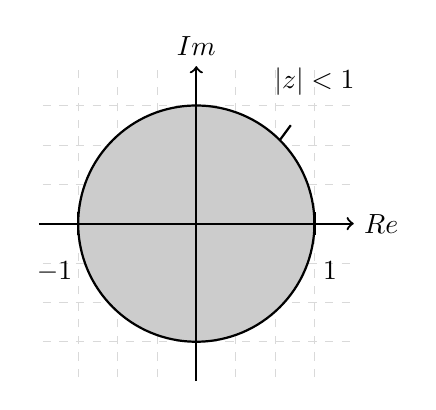
\begin{tikzpicture}[thick,scale=0.5]
\draw[help lines, color=gray!30, dashed] (-3.9,-3.9) grid (3.9,3.9);
\draw (2.12,2.12) -- (2.4,2.5);
 \fill[gray!40,even odd rule, dashed] (0,0) circle (3cm);
   \draw (0, 0) circle (3cm) node[above,xshift=1.5cm,yshift=1.5cm]{$|z|<1$};
\draw[thick] (3,-0.3) -- (3,0.3) node[below,xshift=0.2cm,yshift=-0.5cm]{$1$};
\draw[->, thick] (-4,0)--(4,0) node[right]{$Re$};
\draw[->, thick] (0,-4)--(0,4) node[above]{$Im$};
\draw[thick] (-3,-0.3) -- (-3,0.3) node[below,xshift=-0.3cm,yshift=-0.5cm]{$-1$};
\end{tikzpicture}

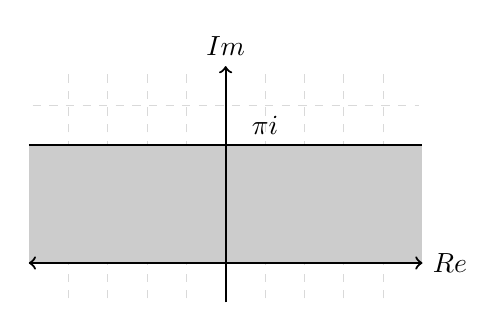
\begin{tikzpicture}[thick,scale=0.5]
\draw[help lines, color=gray!30, dashed] (-4.9,-0.9) grid (4.9,4.9);
 \fill[gray!40,even odd rule] (-5,0) rectangle (5,3);
 \draw[thick] (-5,3)--(5,3)  node[above,xshift=-2cm]{$\pi i$};
\draw[<->, thick] (-5,0)--(5,0) node[right]{$Re$};
\draw[->, thick] (0,-1)--(0,5) node[above]{$Im$};
\end{tikzpicture}
\begin{tikzpicture}
\draw[color=red!10] (-1,0) rectangle (0.5,1);
\draw[thick,->] (-1,2) -- (0,2) node[above,xshift=-0.5cm]{$e^z$};
\end{tikzpicture}
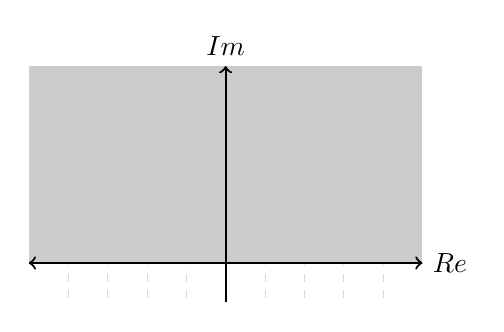
\begin{tikzpicture}[thick,scale=0.5]
\draw[help lines, color=gray!30, dashed] (-4.9,-0.9) grid (4.9,4.9);
 \fill[gray!40,even odd rule] (-5,0) rectangle (5,5);
\draw[<->, thick] (-5,0)--(5,0) node[right]{$Re$};
\draw[->, thick] (0,-1)--(0,5) node[above]{$Im$};
\end{tikzpicture}

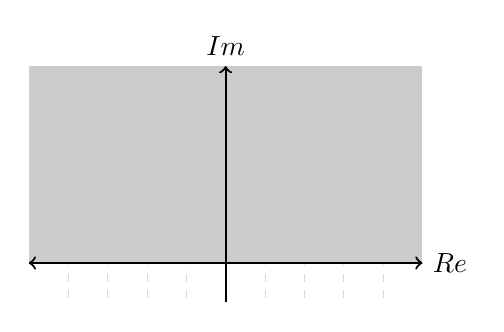
\begin{tikzpicture}[thick,scale=0.5]
\draw[help lines, color=gray!30, dashed] (-4.9,-0.9) grid (4.9,4.9);
 \fill[gray!40,even odd rule] (-5,0) rectangle (5,5);
\draw[<->, thick] (-5,0)--(5,0) node[right]{$Re$};
\draw[->, thick] (0,-1)--(0,5) node[above]{$Im$};
\end{tikzpicture}
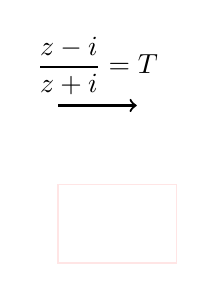
\begin{tikzpicture}
\draw[color=red!10] (-1,0) rectangle (0.5,1);
\draw[thick,->] (-1,2) -- (0,2) node[above,xshift=-0.5cm]{$\displaystyle\frac{z-i}{z+i}=T$};
\end{tikzpicture}
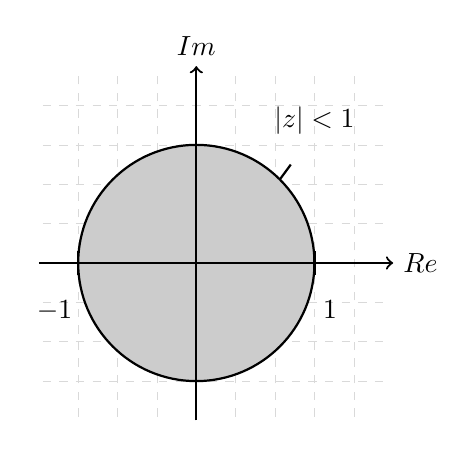
\begin{tikzpicture}[thick,scale=0.5]
\draw[help lines, color=gray!30, dashed] (-3.9,-3.9) grid (4.9,4.9);
\draw (2.12,2.12) -- (2.4,2.5);
 \fill[gray!40,even odd rule, dashed] (0,0) circle (3cm);
   \draw (0, 0) circle (3cm) node[above,xshift=1.5cm,yshift=1.5cm]{$|z|<1$};
\draw[thick] (3,-0.3) -- (3,0.3) node[below,xshift=0.2cm,yshift=-0.5cm]{$1$};
\draw[->, thick] (-4,0)--(5,0) node[right]{$Re$};
\draw[->, thick] (0,-4)--(0,5) node[above]{$Im$};
\draw[thick] (-3,-0.3) -- (-3,0.3) node[below,xshift=-0.3cm,yshift=-0.5cm]{$-1$};
\end{tikzpicture}

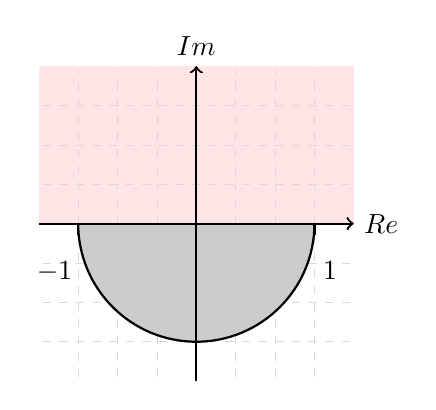
\begin{tikzpicture}[thick,scale=0.5]
\draw[help lines, color=gray!30, dashed] (-3.9,-3.9) grid (3.9,3.9);
\draw (2.12,2.12) -- (2.4,2.5);
 \fill[gray!40,even odd rule, dashed] (0,0) circle (3cm);
   \draw (0, 0) circle (3cm);
\draw[thick] (3,-0.3) -- (3,0.3) node[below,xshift=0.2cm,yshift=-0.5cm]{$1$};
\draw[thick] (-3,-0.3) -- (-3,0.3) node[below,xshift=-0.3cm,yshift=-0.5cm]{$-1$};
\fill[red!10] (-4,4) rectangle (4,0);
\draw[help lines, color=gray!30, dashed] (-3.9,3.9) grid (3.9,0);
\draw[->, thick] (-4,0)--(4,0) node[right]{$Re$};
\draw[->, thick] (0,-4)--(0,4) node[above]{$Im$};
\end{tikzpicture}
\begin{tikzpicture}
\draw[color=red!10!] (-1,0) rectangle (0.5,1);
\draw[thick,->] (-1,2) -- (0,2) node[above,xshift=-0.5cm]{$\displaystyle i\frac{z+1}{-z+1}=T^{-1}$};
\end{tikzpicture}
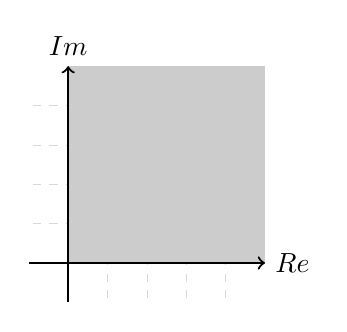
\begin{tikzpicture}[thick,scale=0.5]
\draw[help lines, color=gray!30, dashed] (-0.9,-0.9) grid (4.9,4.9);
 \fill[gray!40,even odd rule] (0,0) rectangle (5,5);
\draw[->, thick] (-1,0)--(5,0) node[right]{$Re$};
\draw[->, thick] (0,-1)--(0,5) node[above]{$Im$};
\end{tikzpicture}
\end{center}

\begin{center}
\hspace{2cm}\begin{minipage}{0.5\textwidth}
\begin{itemize}
\renewcommand\labelitemi{\faBug}
    \item $z^2$ doubles angles,
    \item $\sqrt{z}$ halves angles,
    \item $iz$ rotates $90^\circ$ counterclockwise
\end{itemize}
\end{minipage}
\end{center}
\end{formula}
%----------------------%
%----------------------%


\end{document}
